\label{subart:fdtd}
Metoda różnic skończonych w~dziedzinie czasu (ang. FDTD - finite-difference time-domain) jest szeroko wykorzystywana w~niniejszej pracy ze względu na możliwości symulowania ośrodków materialnych opisywanych modelem Lorenza-Drudego \ref{subart:lorenz-drude}, oraz bezpośrednie obliczanie wartości pól $E$ i~$H$ we wszystkich punktach siatki obliczeniowej. Poniżej przedstawione zostały podstawowe elementy tej metody symulacji numerycznych.
Podstawą do współcześnie prowadzonych symulacji elektromagnetycznych w~dziedzinie czasu jest algorytm Yee\cite{1966ITAP14302Y}, który rozwiązywanie równań Maxwella sprowadza do następującej sekwencji:
\begin{enumerate}
\item Zastąpienie wszystkich pochodnych cząstkowych w~prawach Ampera i~Faradaya różnicami skończonymi.
\item Przekształcenie powstałych równań, tak aby wyrazić amplitudy pól $E$ i~$H$ w~nieznanym czasie $t_0 +  \Delta_t$ przez ich wartości w~czasie $t_0$, oraz wartości drugiego pola w~czasie $t_0+ \frac{\Delta_t}{2}$.
\item Obliczenie wartości pola $H$ w~czasie $t_0 +  \Delta_t$.
\item Obliczenie na podstawie wartości $H$ dla $t=t_0+  \Delta_t$, wartości pola $E$ w~czasie $t_0 + \frac{3}{2} \Delta_t$.
\item Powtarzanie kroków 3-4 w celu ewolucji stanu układu przez żądany czas.
\end{enumerate}
Działanie algorytmu Yee zostanie teraz przedstawione bardziej szczegółowo na przykładzie, który pozwoli nam lepiej zrozumieć te kilka abstrakcyjnie opisanych kroków. Ponieważ prowadzenie rachunków dla problemu trójwymiarowego byłoby przesadnie skomplikowane, dla celów poglądowych skupimy się na zagadnieniu jednowymiarowym.

\subsection{FDTD w~jednym wymiarze}

Załóżmy, że pole elektryczne posiada jedynie składową w~kieruku $z$, w~jedowymiarowej przestrzeni opisywanej przez oś x ($\vec{E}=E_z \cdot \hat{e_z}$). W takiej sytuacji prawo Faradaya możemy zapisać jako:
\begin{equation}
\mu \frac{\partial \vec{H}}{\partial t}= \mu \frac{\partial H_y}{\partial t} \hat{e_y}= \nabla \times \vec{E} = - \frac{\partial E_z}{\partial x} \hat{e_y} 
\label{eq:fdtd-faraday}
\end{equation}
Zgodnie z~oczekiwaniami jedyną zmienną w~czasie składową natężenia pola magnetycznego jest $H_y$. Wykorzystując ten fakt możemy również uprościć zapis prawa Ampera:
\begin{equation}
\varepsilon \frac{\partial \vec{E}}{\partial t}=\nabla \times \vec{H} = \frac{\partial H_y}{\partial x} \hat{e_z}
\label{eq:fdtd-amper}
\end{equation}
Z powyższych równań możemy wyznaczyć skalarny układ równań różniczkowych na składowe $H_y$ i~$E_z$,
\begin{equation}
\mu \frac{\partial H_y}{\partial t}=\frac{\partial E_z}{\partial x} ,
\varepsilon \frac{\partial E_z}{\partial t}=\frac{\partial H_y}{\partial x},
\end{equation} w~którym zmiana w~czasie amplitudy jednego z~pól wyrażona jest przez pochodną względem $x$ drugiego pola. Równanie wyprowadzone z~(\ref{eq:fdtd-faraday}) posłuży nam do wyznaczenia zmiany w~czasie natężenia pola magnetycznego, natomiast równanie~(\ref{eq:fdtd-amper}) do obliczenia przyszłych (w czasie $t_0 + \Delta_t$) wartości pola $E$.

\begin{figure}[tb]
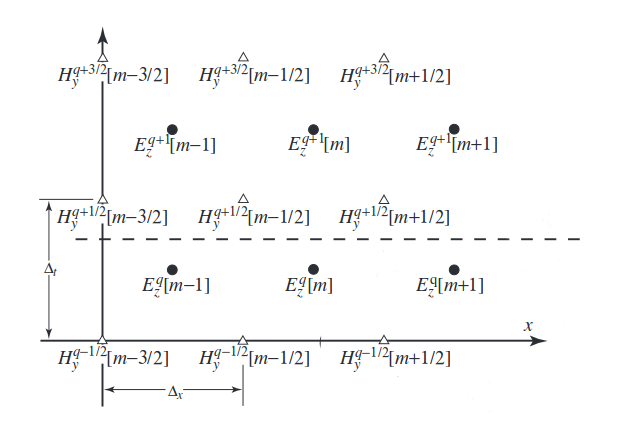
\includegraphics[width=.9\textwidth]{subart/fdtd/leapfrog.png}
\caption{Graficzna prezentacja dyskretyzacji w~jednowymiarowej metodzie FDTD. Pozioma przerywana linia wskazuje przykładową granicę pomiędzy wartościami już obliczonymi i~szukanymi w~kolejnym kroku symulacji. }
\label{pic:leapfrog}
\end{figure}

 Wprowadzając konwencję przypiswania górnych indeksów $q$  iteracjom algorytmu oraz umieszczanych w~nawiasach kwadratowych indeksów m opisujących położenie w~przestrzeni, możemy wyprowadzić formuły na wartości obu pól
\begin{equation}
H_y^{q+\frac{1}{2}}[m+\frac{1}{2}]=H_y^{q-\frac{1}{2}}+\frac{\Delta_t}{\mu \Delta_x}(E^q_z[m+1]-E^q_z[m]),
\label{eq:numhy-1dfdtd}
\end{equation}

\begin{equation}
E_z^{q+1}[m]=E_z^{q}+\frac{\Delta_t}{\varepsilon \Delta_x}(H^{q+\frac{1}{2}}_z[m+\frac{1}{2}]-H^{q-\frac{1}{2}}_z[m-\frac{1}{2}]),
\label{eq:numez-1dfdtd}
\end{equation}
 Ponieważ wartości obu pól w~kolejnym kroku czasowym wyrażane są jedynie przez wartość tego pola w~kroku poprzednim, oraz wartości drugiego pola w~sąsiednich punktach, możemy zastosować dyskretyzację skokową\footnote{Często spotykana jest również nazwa żabi skok, będąca kalką językową z~angielskiego leap-frog}. Jej zastosowanie powoduje, że obliczane wartości pól $E$ i~$H$ nie dotyczą dokładnie tej samej chwili czasu, przez co dokładne uzgodnienie fazy obu pól wymaga wykonania dodatkowego ,,połówkowego'' kroku na jednym z~pól. Zaletą takiej dyskretyzacji jest natomiast wyższa - drugiego rzędu, dokładność numeryczna. Ze względu na zysk numeryczny, algorytm skokowy stosujemy również do dyskretyzacji względem położenia. Graficzną reprezentację rozwiązywania jednowymiarowego problemu elektromagnetycznego metodą FDTD przedstawia rysunek \ref{pic:leapfrog}.

Współczynniki $\frac{\Delta_t}{\varepsilon \Delta_x}$ i~$\frac{\Delta_t}{\mu \Delta_x}$ odgrywają kluczową rolę w~równaniach (\ref{eq:numhy-1dfdtd}) i~(\ref{eq:numez-1dfdtd}). Wygodnie jest przedstawić je w~formie pozwalającej przeanalizować jak daleko energia może propagować się w~pojedynczym kroku czasowym \cite{understanding-fdtd}. W tym celu wprowadza się tzw. współczynnika Couranta, $S=\frac{c \Delta_t}{\Delta_x}$, będący stosunkiem odległości pokonywanej przez front fali elektromagnetycznej w~jednym kroku czasowym i~gęstości próbkowania w~przestrzeni. W przypadku symulacji jednowymiarowych, uwzględniając fakt, że wartości w~kolejnych chwilach czasu zależą jedynie od punktów dyskretnych z~najbliższego otoczenia możemy stwierdzić, że współczynnik Couranta powinien spełniać warunek $S\le1$. W szczególności optymalnym dla omawianej sytuacji jest wybranie $S=1$, ponieważ wtedy w~jednym kroku czasowym front fali elektromagnetycznej pokonuje odległość równą $\Delta_x$. Wybranie właściwego współczynnika Couranta komplikuje wprowadzenie niejednorodności w~obszarze symulacji. Ponieważ prędkość fazowa zależy od współczynnika załamania, przy zachowaniu równomiernego próbkowania przestrzennego doprowadzenie do idealnego dopasowania siatki przestrzennej i~kroku czasowego może okazać się niemożliwe, co prowadzi do powstania ,,dyspersji numerycznej'' na siatce FDTD. 

W ogólności dla problemów wielowymiarowych stosuje się wzór
\begin{equation}
S\le\frac{n_{min}}{\sqrt{DIM}},
\label{eq:courant}
\end{equation}
gdzie przez $DIM$ oznaczono liczbę wymiarów przestrzennych symulacji, a $n_{min}$ najniższy współczynnik załamania materiału znajdującego się w~przestrzeni symulacji. Wyznaczenie odpowiedniego współczynnik Couranta dla symulacji z~materiałami dyspersyjnymi (szerzej omówionymi w~części \ref{subart:lorenz-drude}) jest zagadanieniem skomplikowanym, wymagającym każdorazowego rozpatrzenia parametrów symylacji.

\subsection{Warunki brzegowe}
Równania (\ref{eq:numhy-1dfdtd}) i~(\ref{eq:numez-1dfdtd}) mogą być oczywiście zastosowane jedynie do punktów nie będących granicą obszaru symulacji. Numeryczne rozwiązanie równania różniczkowego zawsze wiąże się z~odpowiednim dobraniem warunków brzegowych, które nie powinny wprowadzać dodatkowych artefaktów do modelowanego zjawiska. Najprosztszym sposobem jest zastosowanie warunku Dirichleta i przyjęcie brzegowych wartości pola elektrycznego lub magnetycznego jako równych 0. Fizycznie wprowadzenie tego typu założenia jest równoważne z~umieszczeniem na granicy symulowanego obszaru idealnego przewodnika, odpowiednio elektrycznego~(PEC)\footnote{Od ang. Perfect Electric Conductor} lub magnetycznego~(PMC)\footnote{Dla wygody numerycznej wprowadza się również przewodniość magnetyczną( W skrócie określanym jako PMC od ang. Perfect Magnetic Conductor)}. Wprowadzenie stałej, równej zero wartości na granicy obszaru symulacji powoduje odbicie obu pól, w~stosunku do pola dla którego ustalono zerową wartość na granicy przy odbiciu następuje zmiana znaku. Przykład wyników symulacji w~pustej przestrzeni ze sztywnymi warunkami brzegowymi znajduje się na ilustracji~\ref{fig:wstep-pml-bad}. Ograniczenie obszaru symulacji za pomocą idealnego przewodnika, de facto ogranicza możliwości metody do modelowania jedynie wnęk rezonansowych. Natomiast większość zjawisk elektromagnetycznych odbywa się w~otwartej przestrzeni \footnote{Za którą z~dobrym przybliżeniem możemy uważać nawet zamknięte laboratorium. Ponieważ analizowane zjawiska dyfrakcji, czy rozpraszania zachodzą w~małym obszarze, położonym z~dala od ograniczeń fizycznych takich jak ściany które słabo odbijają światło widzialne.}.

W przypadku niektórych struktur istnieje naturalne zakończenie obszaru symulacji. Przykładem mogą być periodyczne kryształy fotoniczne, dla których obszar symulacji stanowi komórka elementarna z~periodycznie zadanymi warunkami brzegowymi. Rozwiązania niektórych problemów elektromagnetycznych szybko zanikają w~przestrzeni, w~związku z~czym zastosowanie odpowiednio dużego obszaru symulacji może umożliwić przeprowadzenie obliczeń. Inne zagadnienia wymagają zamiany zmiennych  jak np. $\hat{x}=\textrm{tanh}(x)$, która prowadzi do zmiany dziedziny symulacji z~$x\in(- \infty; + \infty)$ na $\hat{x}\in(-1;1)$ i~rozwiązania zmienionego problemu. 

Wygodniejszym rozwiązaniem pozwalającym na skończonej siatce modelować zjawiska zachodzące w~nieograniczonej przestrzeni, jest wprowadzenie absorpcyjnych warunków brzegowych~ABC (ang. absorbing boundary condition). W przypadku symulacji jednowymiarowej dla $n=1$, dla współczynnika Couranta $S=1$ i~przy zastosowaniu standardowego założenia o~braku źródeł poza obszarem symulacji, tego typu warunek brzegowy można łatwo zrealizować. Wartość amplitudy pola w~węźle na brzegu w~kroku $q+1$ musi być równa amplitudzie tego pola w~kroku $q$ w~węźle sąsiednim. W sytuacji wielowymiarowej, gdy w~obszarze symulacji występują np. materiały stratne~(o zespolonej przenikalności elektrycznej) zagadnienie to staje się znacznie bardziej skomplikowane. Przykładowymi propozycjami rozwiązań omawianego problemu są warunki brzegowe typu TFSF~(ang.~Total Field Scattered Field).

\subsection{Nieodbijające warunki brzegowe (PML)}
\label{art:pml}
Zmianę podejścia do realizacji symulacji numerycznych dotyczących zjawisk w~nieograniczonej przestrzeni zaproponował Jean-Pierre B\'{e}renger~\cite{1994JCoPh.114..185B}. Zamiast konstruowania odpowiedniego warunku brzegowego zaproponował on wprowadzenie nieodbijającej warstwy absorpcyjnej, określanej jako PML~(ang.~perfectly matched layer), przylegającej do granicy obszaru symulacji. Dzięki zastosowaniu takiej warstwy, za nią możemy użyć np.~warunków Dirichleta, ponieważ po przejściu przez warstwę PML natężenie pola E-M będzie na tyle słabe, że fala odbita od brzegu nie będzie miała wpływu na wynik symulacji. Warstwa PML tworzona jest ze sztucznego materiału, którego własności zostały wyprowadzone przez podział rozwiązania równania falowego,  stąd stosowana angielska nazwa {\it split-field} PML.\footnote{Orginalne wyprowadzenie podane przez B\'{e}rengera dotyczyło rozwiązywania równań Maxwella. To samo podejście zostało jednak bezpośrednio przełożone na modelowanie innych zjawisk opisywanych równaniem falowym.}.  Wyprowadzenie podane przez B\'{e}rengera  wymagało również wprowadzenia do równań Maxwella przewodnictwa magnetycznego, które było niezerowe jedynie w~niefizycznym obszarze PML.


\begin{figure}[tb]
	\centering
	\begin{subfigure}{0.45\textwidth}
		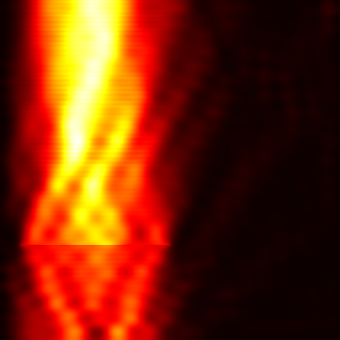
\includegraphics[width=\textwidth]{images/wstep/SUM-nopml-energy.png}
		\caption{}
		\label{fig:wstep-pml-bad}
	\end{subfigure}
	\begin{subfigure}{0.45\textwidth}
		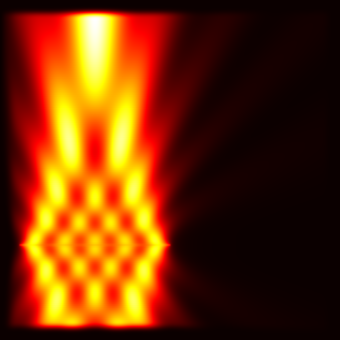
\includegraphics[width=\textwidth]{images/wstep/SUM-pml-energy.png}
		\caption{}
	\end{subfigure}
	\caption{Porównanie wyników symulacji z~propagacją fali E-M w~wolnej przestrzeni dla symulacji w~której brzeg z~warunkiem Dirichleta (a) jest otaczany przez materiał o~$n=1$ , (b) został otoczony obszarem PML}
\end{figure}

Obecnie powszechnie wykorzystywana jest wersja PML nie wymagająca modyfikacji równania falowego, która wyraża PML przez obszar symulacji zajmowany przez jednoosiowy absorbujący materiał anizotropowy. Stąd stosowana nazwa UPML~(ang. uniaxial PML). Pierwotne wyprowadzenie UPML oparte było na analitycznym obliczeniu własności materiału spełniającego warunki absorpcyjności i~zerowego współczynnika odbicia, niezależnie od polaryzacji i~kąta padającego promieniowania E-M  \cite{sacks1995perfectly}. Później przedstawione zostały bardziej elegancie formy wyprowadzenia PML oparte na optyce transformacyjnej~\cite{rappaport1995perfectly}. Podobne wyprowadzenie UPML przytoczone jest w~rozdziale \ref{roz:pml} niniejszej pracy.

Należy również nadmienić, że PML posiada pewne ograniczenia. Jednym z~nich jest zależność współczynnika absorpcji od kąta padania promieniowania E-M. Współczynnik tłumienia jest proporcjonalny do $k_0 \textrm{cos}(\theta)$, gdzie $\theta$ jest kątem padania. Dla kątów bliskich $\frac{\pi}{2}$ tłumienie fali padającej dąży do zera, w~związku z~czym takie fale będą w~znacznym stopniu docierać do brzegu symulacji po odbiciu. W praktyce, w~symulacjach FDTD można uniknąć tego typu problemów zapewniając odpowiednią odległość symulowanego układu od obszaru PML.


Zasadniczym problemem dotyczącym PML w~symulacjach numerycznych jest odbicie na granicy PML wynikające z~dyskretności siatki obliczeniowej. W celu uniknięcia problemów związanych z~odbiciem numerycznym stosowany w~obliczeniach PML nie jest jednolitym ośrodkiem, ale składa się z~wielu warstw ośrodków o~coraz to większym współczynniku absorpcji.

Niedoskonałością PML, której w~żaden sposób nie można uniknąć jest założenie o~jednorodności ośrodka graniczącego z~PML w~kierunku prostopadłym do PML. Rozwiązaniem pozwalającym uniknąć odbić w~sytuacji, gdy to założenie nie jest spełnione, jest wykorzystanie jedynie absorberów opartych na twierdzeniu adiabatycznym~\cite{oskooi2008failure}.

\subsection{Źródła pola elektromagnetycznego w~symulacjach metodą FDTD}
Ostatnim z~omawianych podstawowych elementów metody FDTD jest wprowadzenie źródeł. Najprostrzym sposobem na realizację tego zadania jest umieszczenie tzw. źródła sztywnego. W takim przypadku w~wybranym punkcie lub punktach symulacji pole elektryczne, nie jest obliczane zgodnie z~równaniem (\ref{eq:numez-1dfdtd}). Zamiast tego zależność pola elektrycznego od czasu jest dla niego podana w~sposób analityczny. Tego typu źródło, podobnie jak zadane w~sposób stały warunki brzegowe wprowadza dodatkowe odbicia w~obszarze symulacji.

Innym sposobem wprowadzenia źródła, jest wykorzystanie prawa Amp\'{e}ra z~gęstością prądu
\begin{equation}
\nabla \times \vec{H} = \vec{J} + \varepsilon \frac{\partial \vec{E}}{\partial t},
\label{eq:amper-j}
\end{equation}
gdzie $\vec{J}$ może być rozumiany jako gęstość prądu elektrycznego związana z~przepływem nośników swobodnych w~materiale o~określonej przewodności elektrycznej $\sigma$, ale może też być wykorzystany jako sposób wprowadzenia źródła pola elektrycznego do symulacji. Wprowadzenie źródła addytywnego wymaga wykorzystania innego równania niż prezentowane wcześniej (\ref{eq:numez-1dfdtd}). Wyprowadzamy je z~(\ref{eq:amper-j}) przez zastąpienie pochodnych różnicami skończonymi podobnie jak w~poprzednim wypadku. 



\subsection{Metoda FDTD dla układów o~symetrii walcowej (BOR-FDTD)}
\label{subart:borfdtd}
W przypadku symulacji dotyczącej struktury o~symetrii cylindrycznej możliwe jest zredukowanie problemu trójwymiarowego do problemu dwuwymiarowego. Po zamianie współrzędnych na cylindryczne w~równaniach (\ref{eq:fdtd-faraday}) i~(\ref{eq:fdtd-amper}), zależność od kąta $\phi$ separuje się od zmiennych przestrzennych $r$ i~$z$ dając analityczne rozwiązanie w~postaci szeregów zależnych od kąta
\begin{equation}
	\begin{gathered}
	\vec{E}(\vec{r},t)=\sum_{m=0}^{\infty}(\vec{e_u}(r,z,t) \textrm{cos}(m\phi)+\vec{e_v}(r,z,t)\textrm{sin}(m\phi)) \\
	\vec{H}(\vec{r},t)=\sum_{m=0}^{\infty}(\vec{h_u}(r,z,t) \textrm{cos}(m\phi)+\vec{h_v}(r,z,t)\textrm{sin}(m\phi)).
	\end{gathered}
	\label{eq:bor-fields}
\end{equation}

W powyższym wzorze $m$ jest liczbą numerującą azymutalne mody pola E-M, dla określonego modu prowadzenie symulacji wymaga jedynie aktualizowania wartości $e_u$,$e_v$,$h_u$~i~$h_v$, które są funkcjami jedynie dwóch zmiennych przestrzennych. Jeżeli rozkład pola na początku symulacji oraz pól generowanych przez źródła znajdujące się w~obszarze symulacji można rozłożyć na skończoną liczbę elementów sum ze wzorów (\ref{eq:bor-fields}). To rozwiązując kilka problemów dwu wymiarowych, a następnie stosując zasadę superpozycji, możemy znaleźć rozwiązanie problemu trójwymiarowego, metodą o~dużo mniejszej złożoności obliczeniowej i~mniejszych wymaganiach pamięciowych\footnote{Liczba punktów w~symulacji dwuwymiarowej jest kwadratową funkcją rozdzielczości, a w~przypadku obliczeń w~trzech wymiarach sześcienną}.

\begin{figure}
	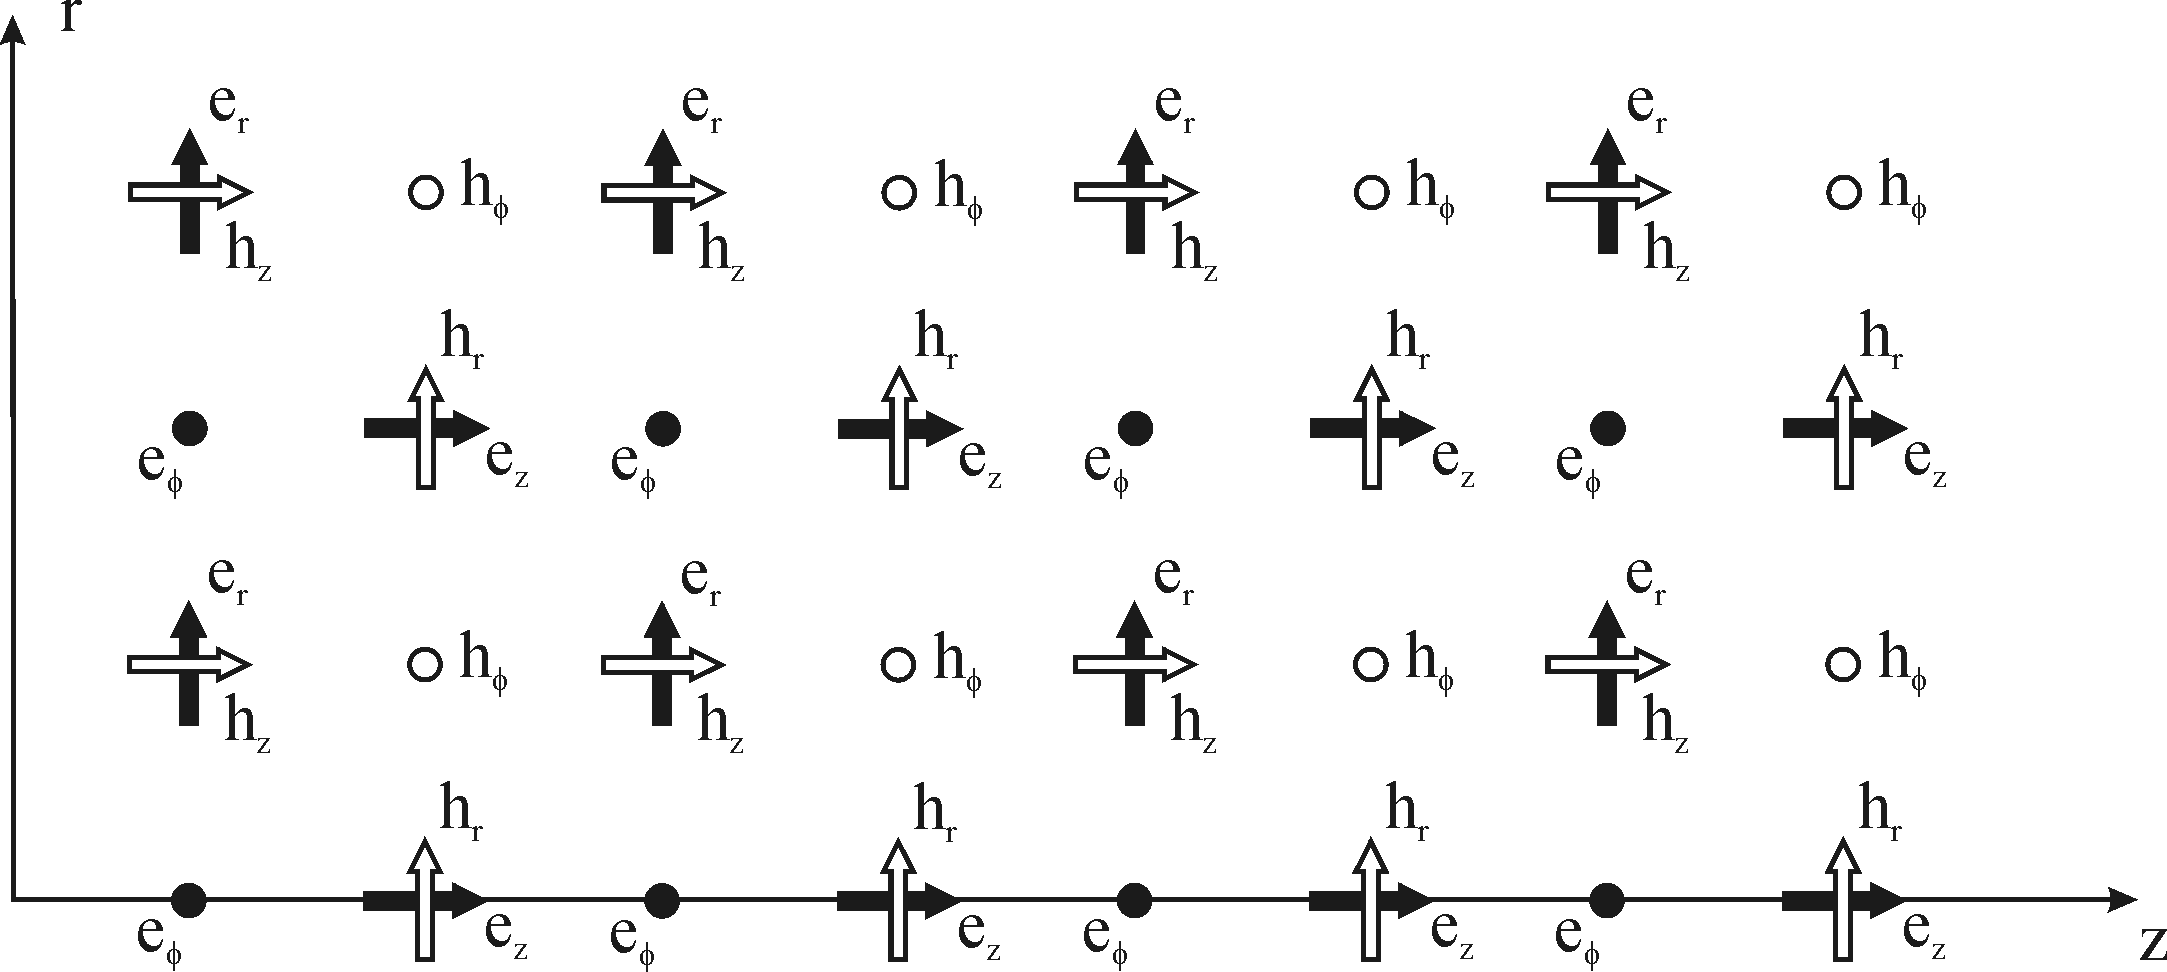
\includegraphics[width=\textwidth]{subart/fdtd/R5_TFSF.png}
	\caption{Przykład dyskretyzacji wykorzystywanej do rozwiązywania równań różniczkowych metodą BOR-FDTD \cite{antosiewicz2009wplyw}}
	\label{fig:bor-dysk}
\end{figure}
W przypadku symulacji BOR-FDTD stabilność numeryczna wyrażana przez współczynnik Couranta zależy od $m$. Dla $m=0$ największa dopuszczalna wartość współczynnika Couranta $S=\frac{n_{min}}{\sqrt{2}}$, gdzie $n_{min}$ oznacza najniższy współczynnik załamania materiałów w~obszarze symulacji. Dla wyższych modów $S \propto m+1$. 

Ze względu na symetrię układu współrzędnych, pola, których punkty dyskretyzacji znajdują się na osi $z$ są tożsamościowo równe zero, $e_z=0$ dla modu $m=0$, oraz $e_{\phi}=0$~i~$h_r=0$ dla m=1 ( dla dyskretyzacji jak na rysunku \ref{fig:bor-dysk}). Ze względu na specjalne traktowanie osi symetrii podczas obliczeń jest to obszar symulacji najbardziej podatny na niestabilności numeryczne. W szczególności, jeśli interesujące nas zjawiska zachodzą z dala od osi optycznej poprawę stabliności uzyskuje się poprzez wymaganie zerowych wartości na kilku rzędach węzłów dyskretyzacji znajdujących się najbliżej osi układu~\cite{OskooiRo10}.

W symulacjach prowadzonych metodą BOR-FDTD wynikowe rozkłady pola są dwuwymiarowymi mapami, na których jedna z~osi odpowiada współrzędnej $z$ - równoległej do osi symetrii. Druga natomiast współrzędnej $r$ - odległości od osi. 
